\section{Introduction}
%%% TODO: add motiviation for cell diffusion models from real world applications 
% intro pp model 
We consider the point particle model on a two dimensional bounded domain $\Omega \subset \mathbb{R}^2$, where we have $N \in \N$ particles and have no real size.
There is also no particle interaction, as there is no possibility of collision. 
Initially, the particles are randomly distributed in $\Omega$. \\
The particles' dynamics are governed solely by Brownian motion.
Brownian motion is a random and unpredictable motion that occurs in the real world when particles are suspended in a fluid and collide with surrounding molecules. \\
In mathematics, we model Brownian motion using stochastic differential equations (SDEs), which are equations that describe the motion of a particle over time in a random and unpredictable manner. 
SDEs are a powerful tool for modeling complex phenomena in physics, finance, and other fields, and are characterized by the presence of random terms that capture the uncertainty of the system. \\
Let 
\[\vec{x}_i(t) \in \Omega \quad 1 \leq i \leq N,\]
be the location of the particle $i$ at time $t > 0$. 
The particle movement can be modeled using the diffusion equation, which describes the random motion of particles over time
\begin{center}
	$d\vec{x}_i(t) = \sqrt{2D} \: dB_t^{(i)}, \quad 1 \leq i \leq N$,
\end{center}
where the constant $D > 0$ represents the diffusion coefficient which proportionally scales the speed of the particle movements by scaling the random fluctuations.
The term $dB_t^{(i)}$ introduces the randomness of Brownian motion, where $dB_t^{(i)}$ is a normally distributed random variable that accounts for the unpredictable changes in the position of particle $vec{x}_i$ over time. \\
We also consider the probability density function $\rho(t, \vec{x})$, which describes the probability of finding a particle at a specific position $\vec{x}$ at time $t$.
In the given context, the function $\rho$ satisfies the partial differential equation:
\begin{align}
	\dfrac{\partial \rho (t, \vec{x})}{\partial t} = D \Delta_{\vec{x}} \rho(t, \vec{x}) \label{eq:pointparticle}, 
\end{align}
where $\Delta_{\vec{x}}$ is the Laplacian operator with respect to the spatial variables. \\
Equation~\eqref{eq:pointparticle} represents the classic diffusion equation, a cornerstone of physics and mathematics.
The same diffusion constant $D>0$ is used in the SDE for particle movement and the PDE for the probability density function $\rho$. \\

% intro hp model 
Next, we consider models that add a real size to the particles and introduce particle interactions. 
With the inclusion of a real size, the particles cannot overlap, resulting in exclusion effects. 
To account for this, we introduce a new interaction dynamics that ensures the particles do not overlap. 
This new interaction dynamics leads to a more complex and realistic model that captures the behavior of particles with a real size and interactions. \\
Since particles cannot overlap, the domain $\Omega^{(i)}_{\epsilon}$, that holds the information where the centre of particle $i$ can be located, must exclude the areas where $\norm[\vec{x}_i - \vec{x}_j] \leq \epsilon$ for all $1 \leq j \leq N,$ $j \neq i$. 
This is due to the fact that particles cannot occupy the same space simultaneously. \\
The domain that holds all possible locations of the particles is then given by \[\Omega^N_{\epsilon} = \Omega^{(1)}_{\epsilon} \times \ldots \times \Omega^{(N)}_{\epsilon} .\] 
This can be visualized as a product space, where each particle's domain is combined to form a larger domain that encompasses all possible locations of the particles.
Under this circumstances, we will get a new dynamic compared to the point particle model.  \\
In the work of Bruna et al. \cite{Bruna2012}, a hard sphere particle model is examined.
Here, the particles are spherical in shape, with a diameter $0 < \epsilon \ll 1$.
All particles in this model are distinct and can be distinguished from one another. \\
The hard sphere model is characterized by the fact that any interaction between particles may cause a change in their direction of motion, but the spherical shape of the particles remains unchanged.
Hardcore collisions are modeled as reflective boundary conditions on the collision surfaces defined by $r = \norm[\vec{x}_i - \vec{x}_j] = \epsilon$, where $1 \leq i < j \leq N$.
The external forces acting on a particle in the system are described by the force function $f: \R^2 \rightarrow \R^2$, which depends only on the location of the particle.
The function $\vec{F}$ maps the particle configuration $\vec{X} = (\vec{x}_1, \ldots, \vec{x}_N)^T$ to the vector of external forces $\vec{F}(\vec{X}) = (f(\vec{x}_1), \ldots, f(\vec{x}_N))^T$.
The dynamics of the particles are governed by the SDE
\begin{center}
	$d\vec{x}_i(t) = \sqrt{2D} \: dB_t^{(i)} + f(\vec{x}_i(t)) \: dt, \qquad 1 \leq i \leq N$.
\end{center}
In this model, the particles are initially randomly distributed in $\Omega^N_{\epsilon}$, ensuring that no overlap occurs between the particles.
The joint probability density function $P$ of the $N$ particles satisfies the high-dimensional Fokker-Planck equation
\begin{center}
	$\dfrac{\partial P}{\partial t} = \nabla_{\vec{X}} \cdot (D \nabla_{\vec{X}} P - P \vec{F})$,
\end{center}
where $\nabla_{\vec{X}}$ and $\nabla_{\vec{X}} \cdot$ denote the gradient and divergence operators with respect to the $N$-particle position vector $\vec{X}$.\\
Using the method of matched asymptotic expansions, the authors also derived the probability density function $\rho$ of finding a single particle at time $t$ and position $\vec{x}$, which satisfies the equation
\begin{align}
	\dfrac{\partial \rho (t, \vec{x})}{\partial t} = \Delta_{\vec{x}} \rho + \alpha_d (N - 1) \epsilon^d \Delta_{\vec{x}} (\rho^2) - \nabla_{\vec{x}} \cdot (f(\vec{x}) \rho).
\end{align}
When $f$ is neglected and $\epsilon \rightarrow 0$, this equation reduces to the probability density function of the point particle model, except for a rescaling factor.
Similarly, the Fokker-Planck equation is a direct extension of the diffusion equation, with an additional drift term.\\

% bachelor intro sp model 
Next, we consider an extension of the model by introducing deformable soft spherical particles. 
This new model incorporates the effect of deformation and interaction between particles through a potential energy function that depends on the distance between the particles.
The paper~\cite{Bruna2017}, written by Bruna, Chapman and Robinson, analyses the diffusion properties of such a model. \\
The equation of motion for each particle $i$ is given by
\begin{equation}
d\vec{x}_i(t) = \sqrt{2D} \: dB_t^{(i)} + f(\vec{x}_i(t))\: dt - \sum\limits_{j\neq i} \nabla_{\vec{x}_i} u (\norm[ \vec{x}_i(t) - \vec{x}_j(t)]) \: dt, \qquad 1 \leq i \leq N,
\end{equation}
where $\nabla_{\vec{x}_i}$ is the gradient with respect to $\vec{x}_i$. \\
The effect of the interaction potential is to cause particles to repel or attract each other depending on the distance between them, rather than simply overlapping. \\
For the modeling of short range interacting soft sphere particles, the authors computed the one particle probability density $\rho(t, \vec{x})$ of finding a given particle at position $\vec{x}$ at time $t$ developing according to
\begin{equation}
\dfrac{\partial \rho}{\partial t} = \nabla_{\vec{x}} \cdot (D \nabla_{\vec{x}} \rho - f(\vec{x}) \rho + \alpha_u \epsilon_u^2(N-1)\rho \nabla_{\vec{x}} \rho)
\end{equation}
where $\alpha_u$ depends on the interaction potential $u$ and $0 < \epsilon_u \ll 1$ is the interaction range of $u$.


%figure for point particles, hard and soft sphere particles, phase field and vertex model
\begin{figure}[t!]
	\centering
	\begin{subfigure}{0.4\textwidth}
		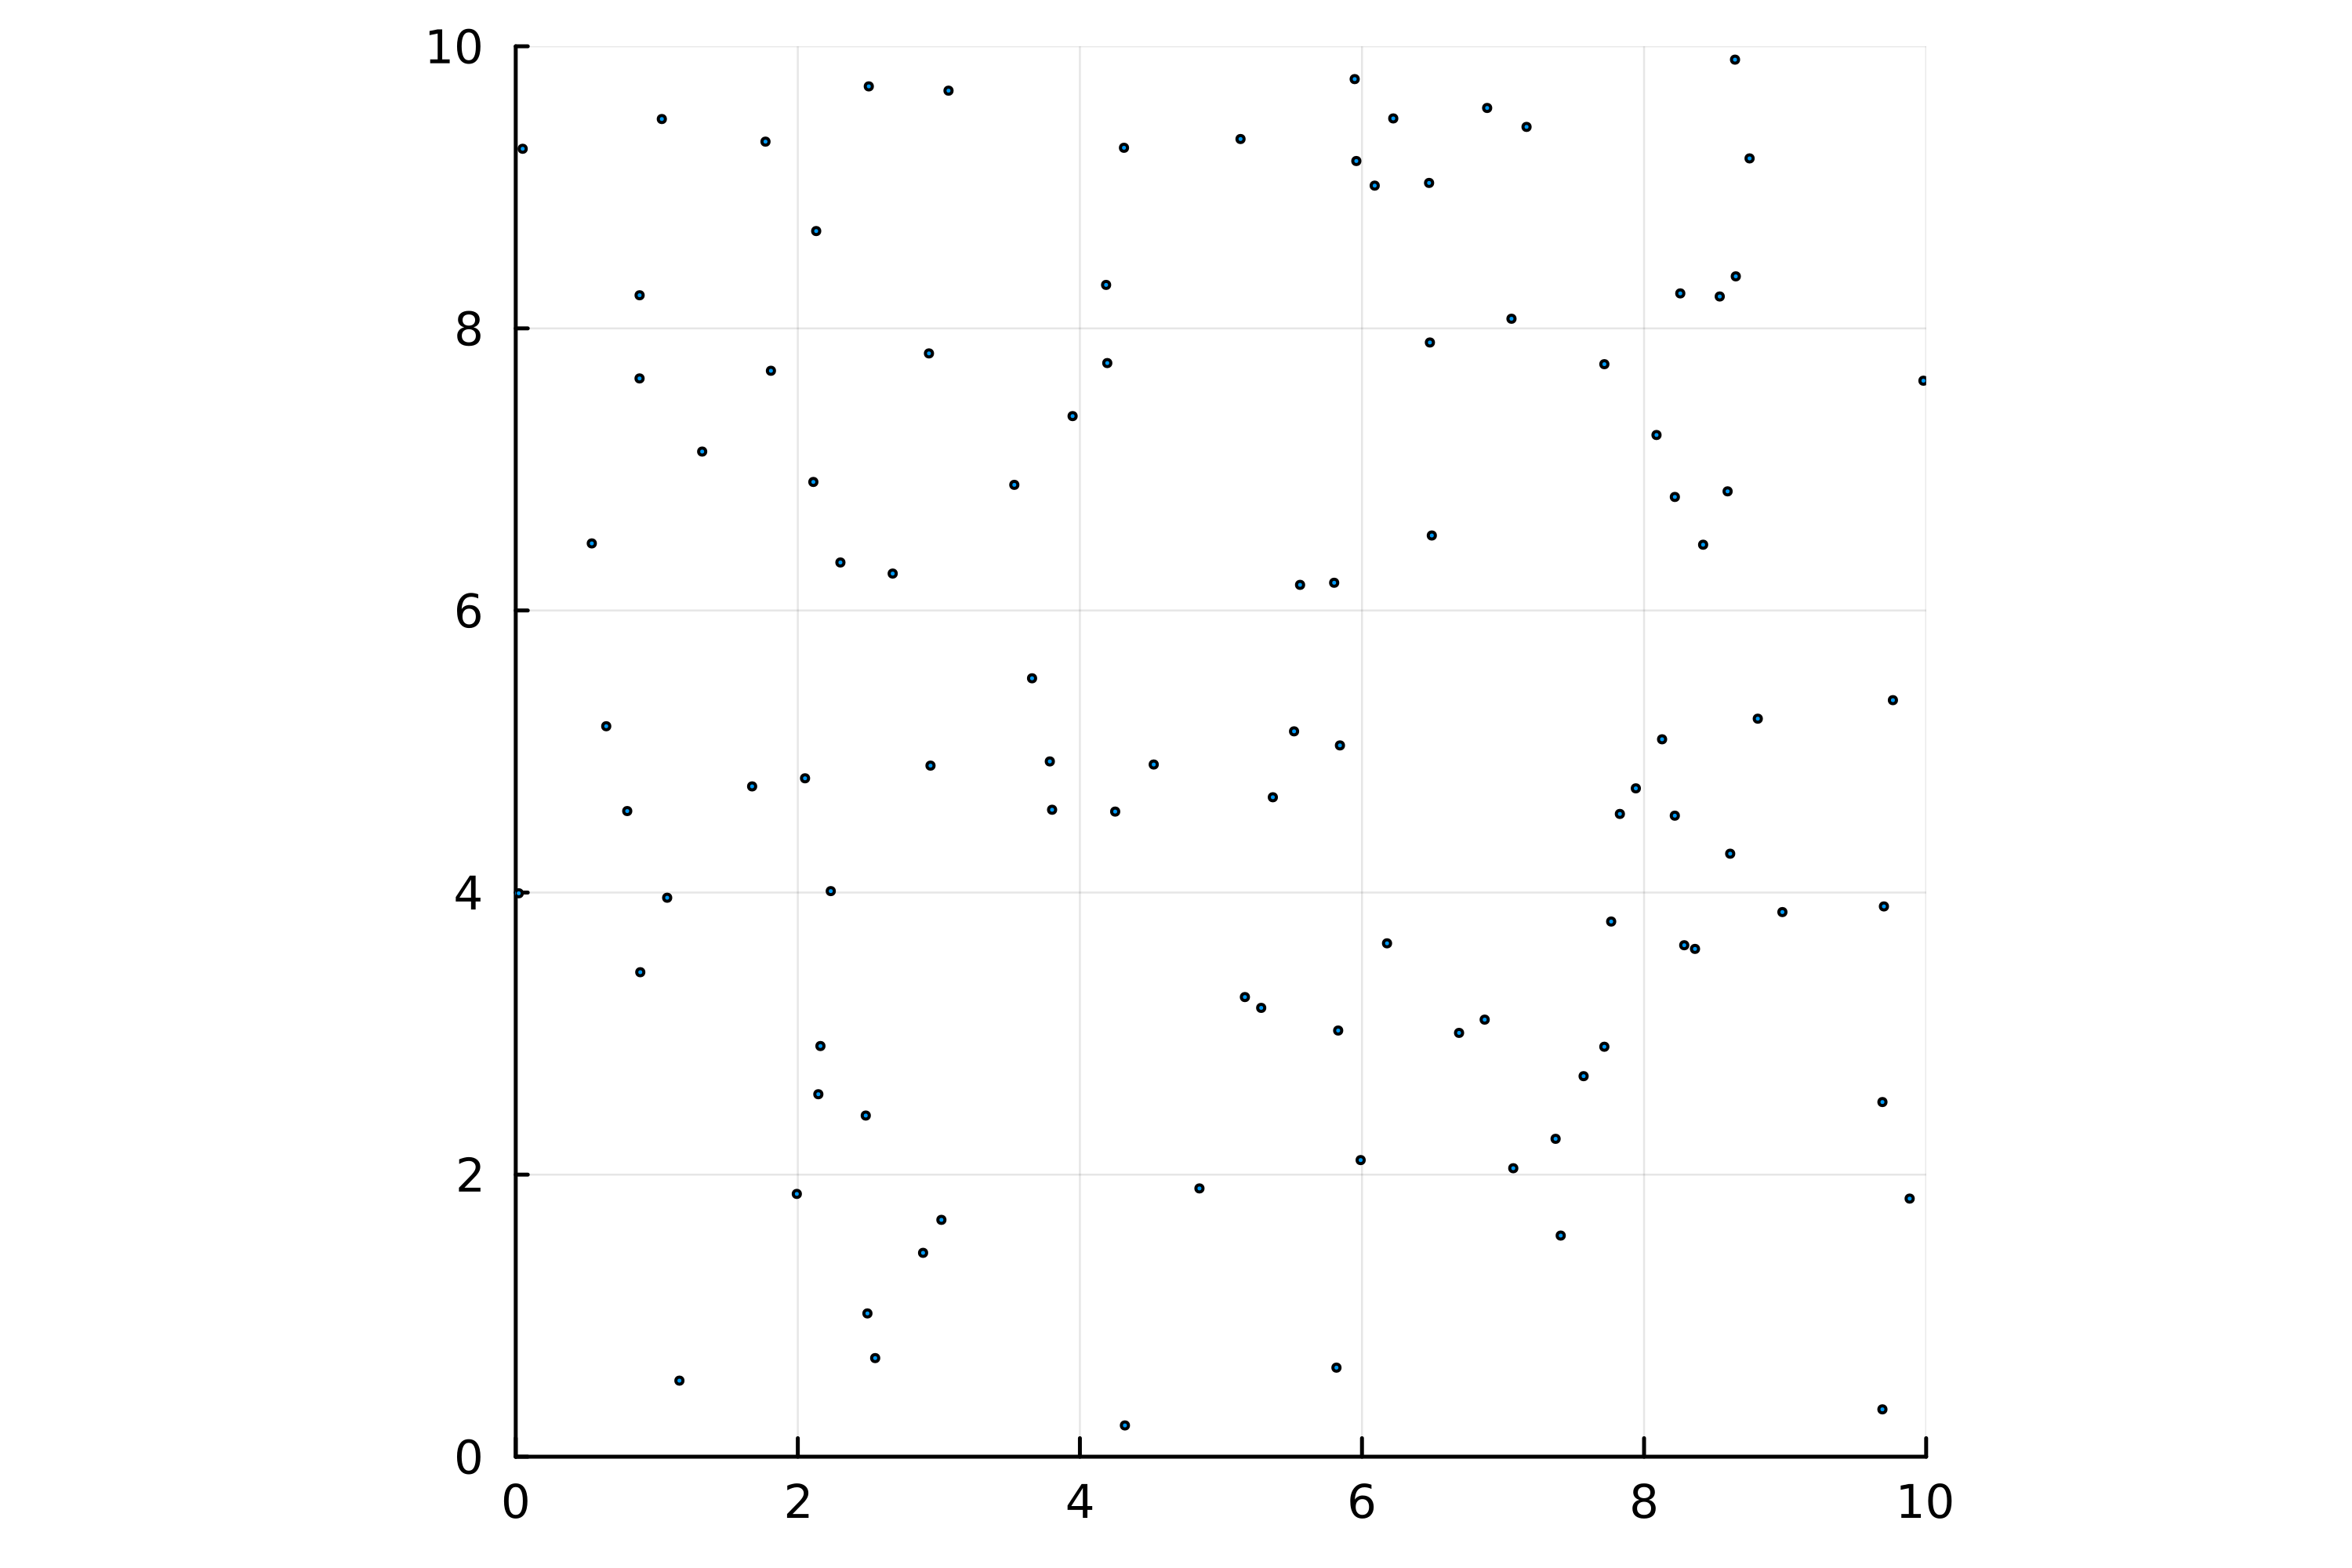
\includegraphics[width=\textwidth]{bachelors-thesis/model_illustrations/particleModel.png}
		\caption{Here, one can see a possible snapshot of the point particle model that is explained at the beginning. 
        The particles are randomly distributed in $\Omega$. 
        The execution of the Brownian motion will cause the particle density to change according to the Diffusion equation.}
	\end{subfigure}
	\hfill
	\begin{subfigure}{0.4\textwidth}
		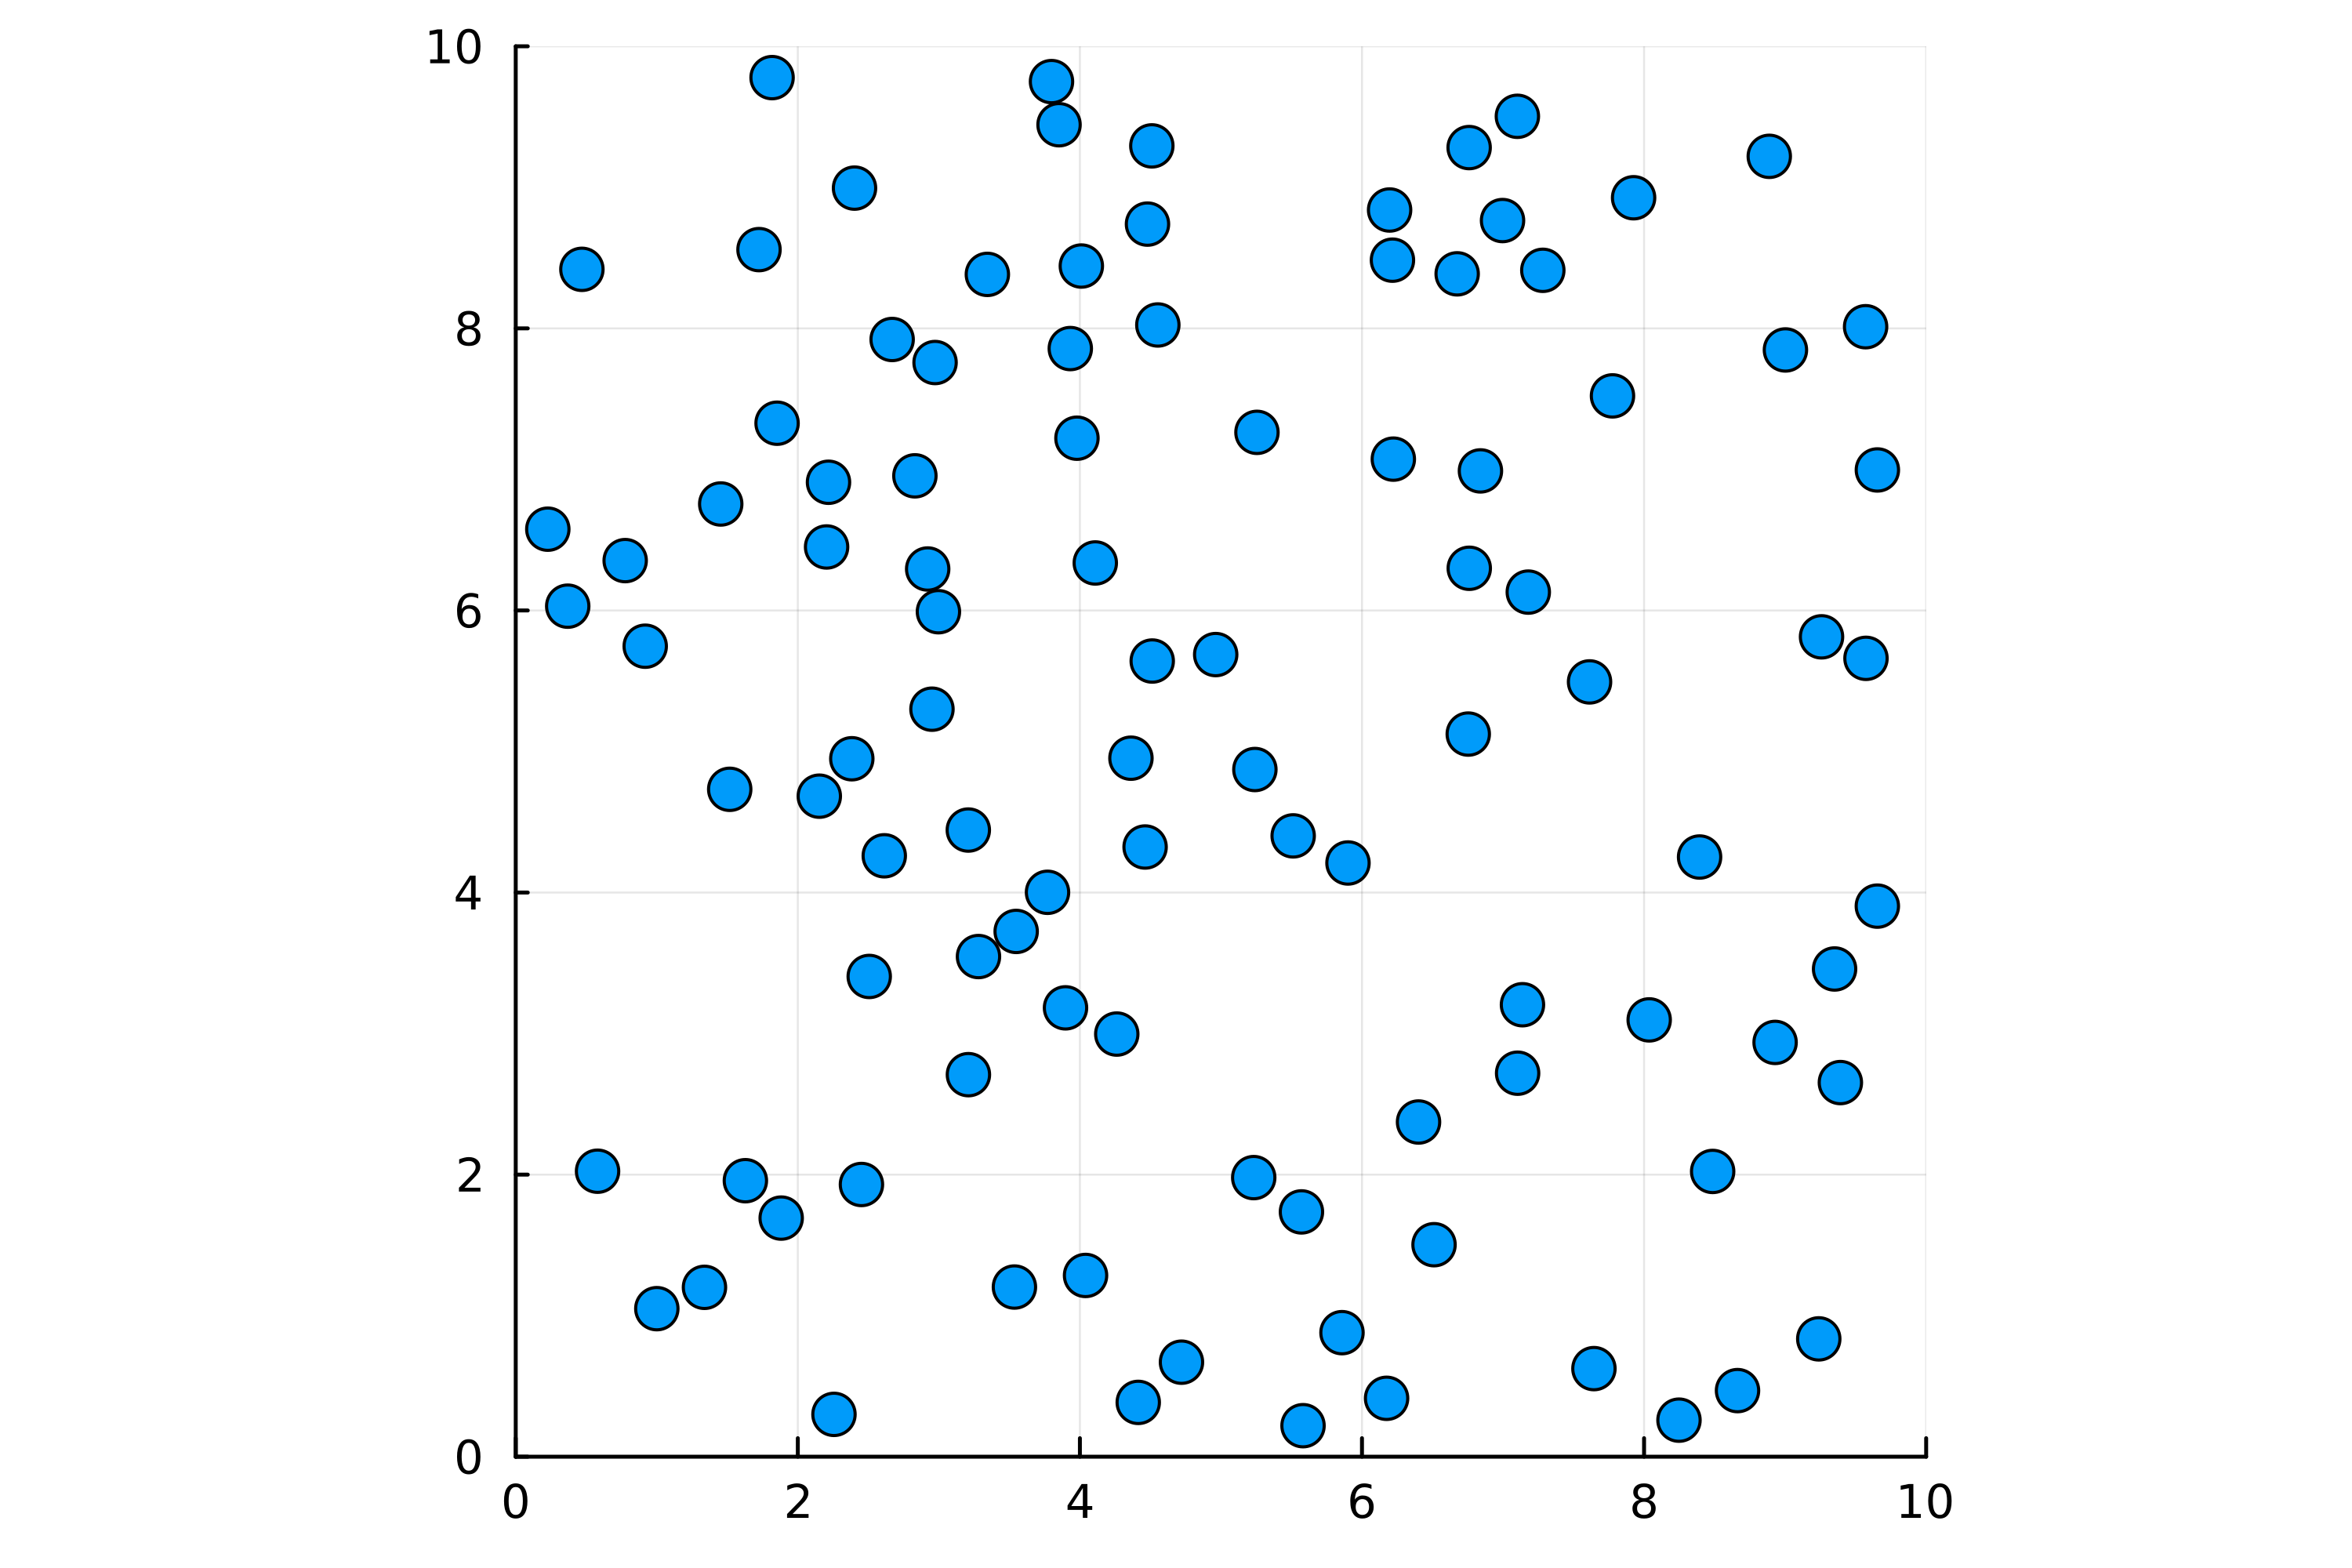
\includegraphics[width=\textwidth]{bachelors-thesis/model_illustrations/SphereModel.png}
		\caption{In contrast to Figure (a), the particles do have a real radius in the sphere models. 
        This causes particle interaction terms as addition in the particle movement, since particles can now collide. 
        The type of interaction terms determines whether it is a hardsphere or softsphere model.   }
	\end{subfigure}
	\hfill
	\begin{subfigure}{0.4\textwidth}
		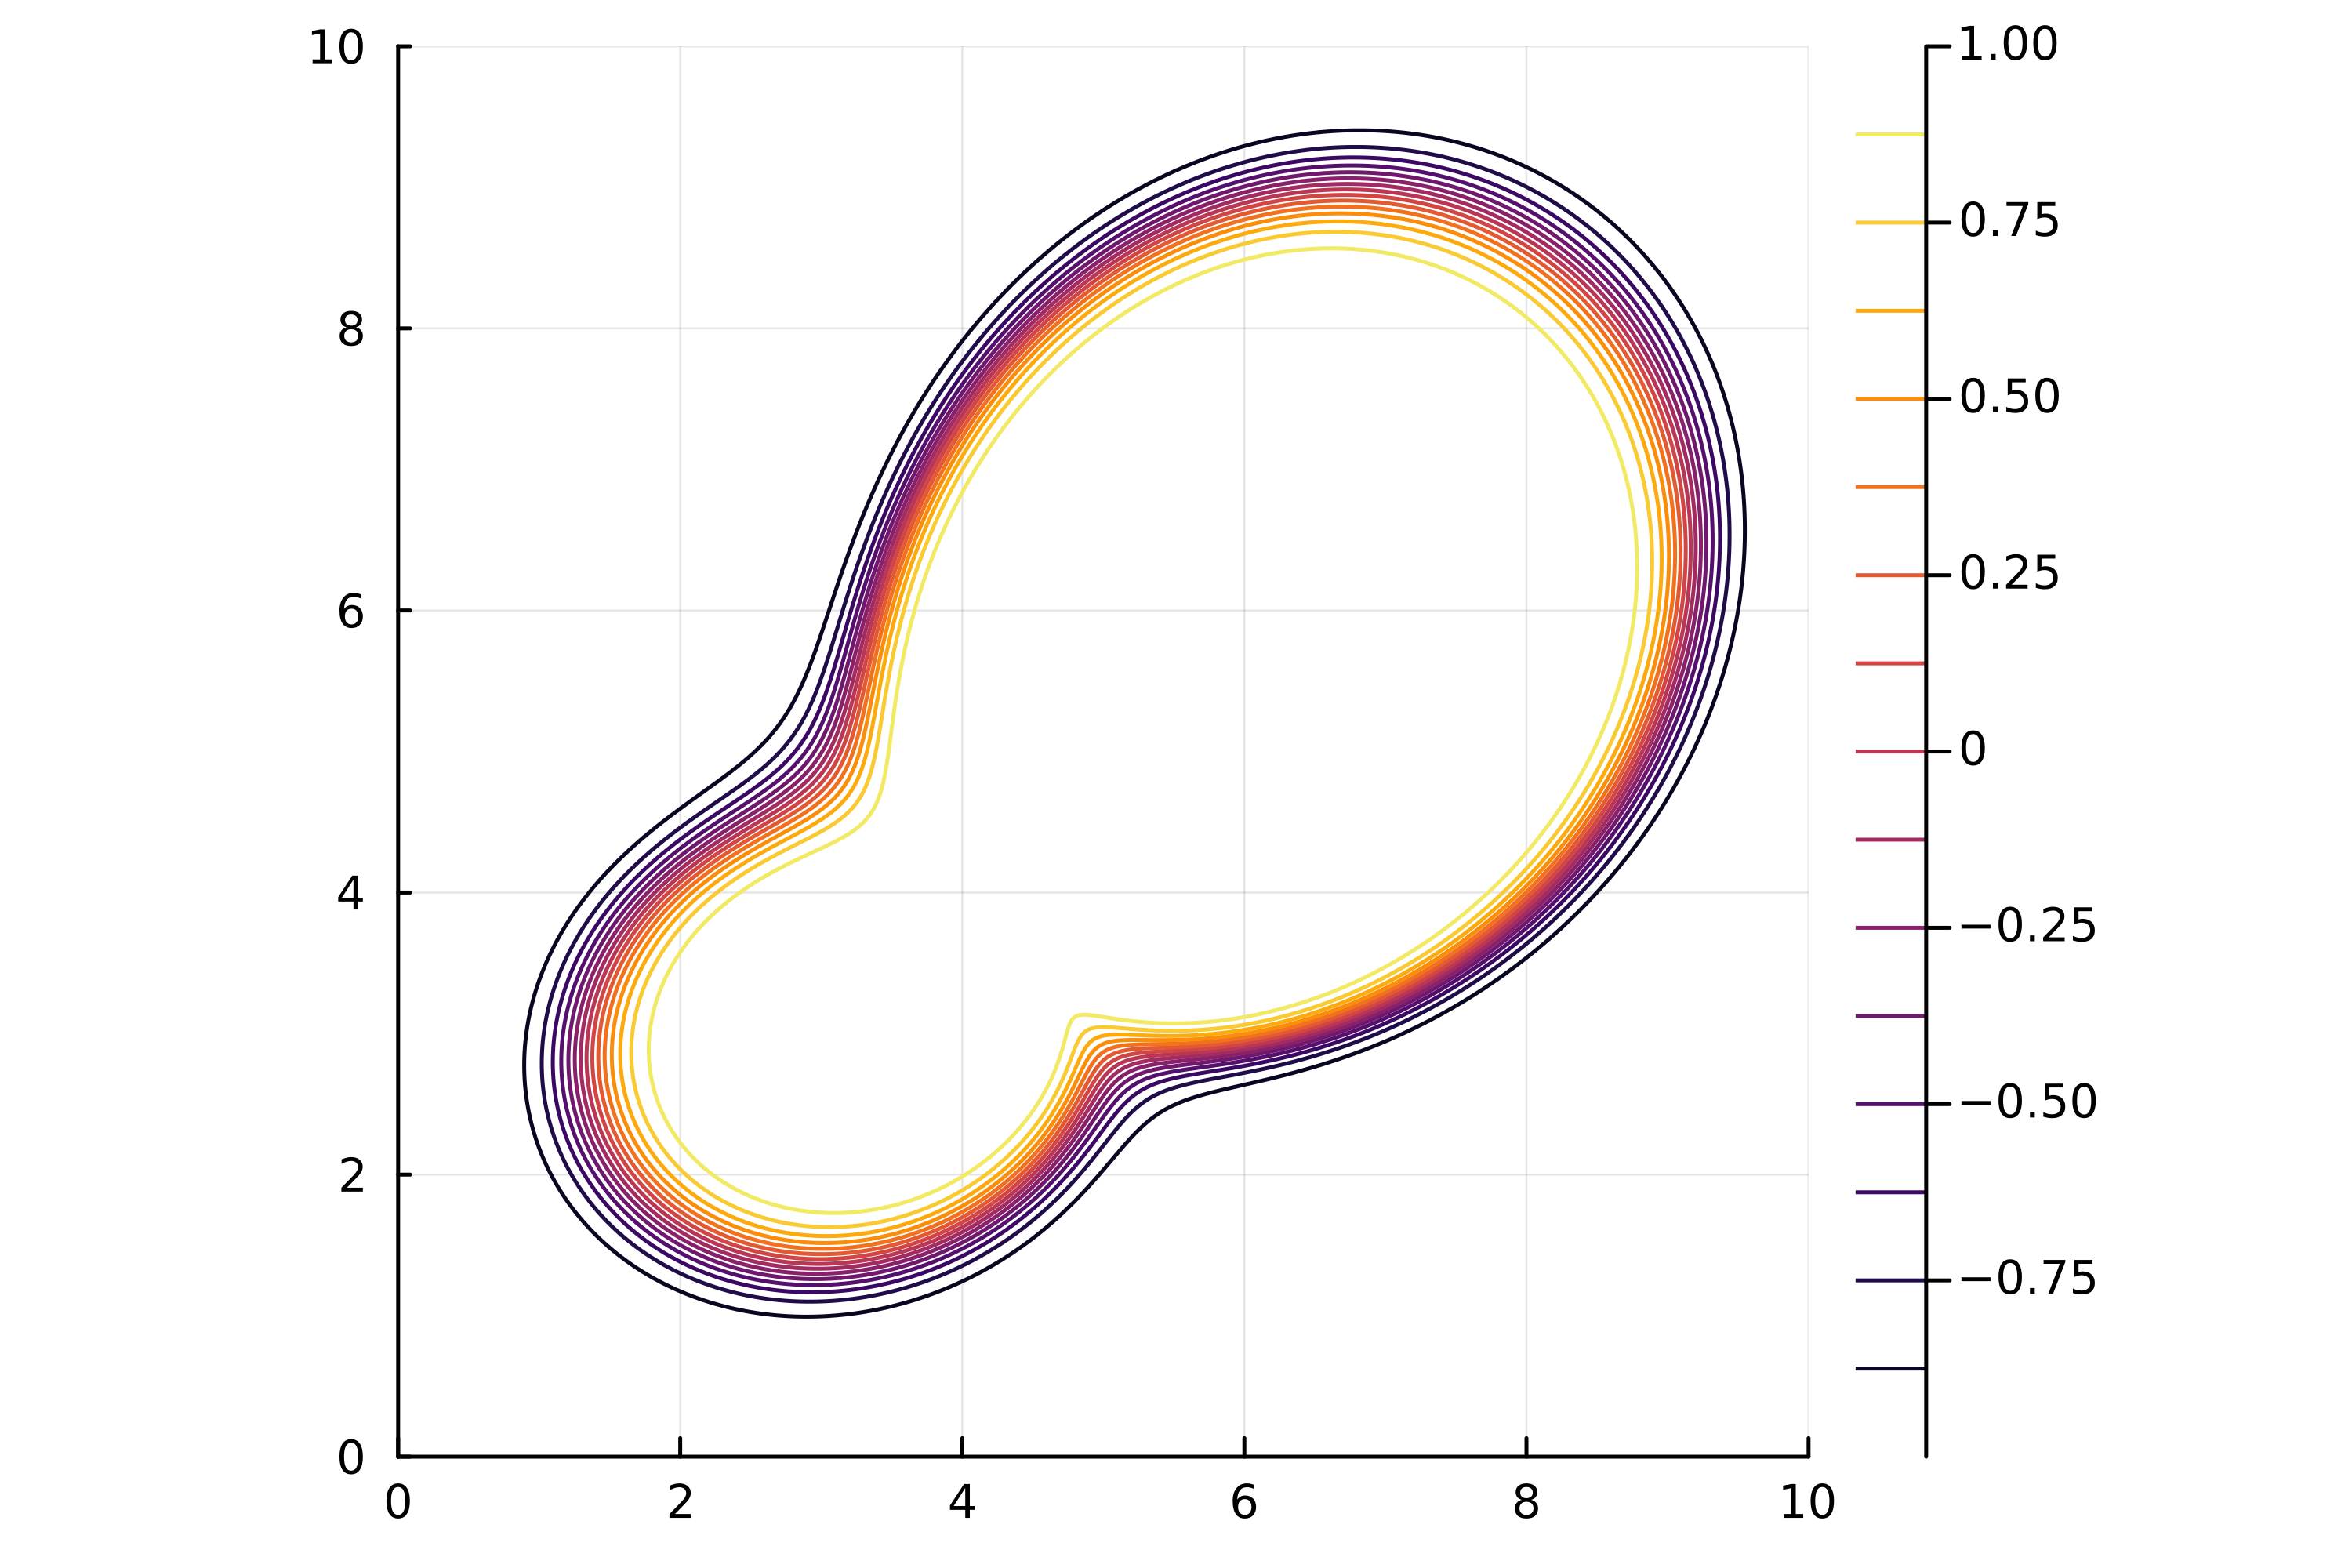
\includegraphics[width=\textwidth]{bachelors-thesis/model_illustrations/PhaseFieldModel.png}
		\caption{A contour plot of a phase field variable $\phi$ illustrates how cells can be modeled through phase field models. 
        The cell's inside is the area where $\phi > 0$. 
        The cell wall sits on the red line where $\phi = 0$. 
        The outer lines display the smooth transition to the outside. }
	\end{subfigure}\hfill
	\begin{subfigure}{0.4\textwidth}
		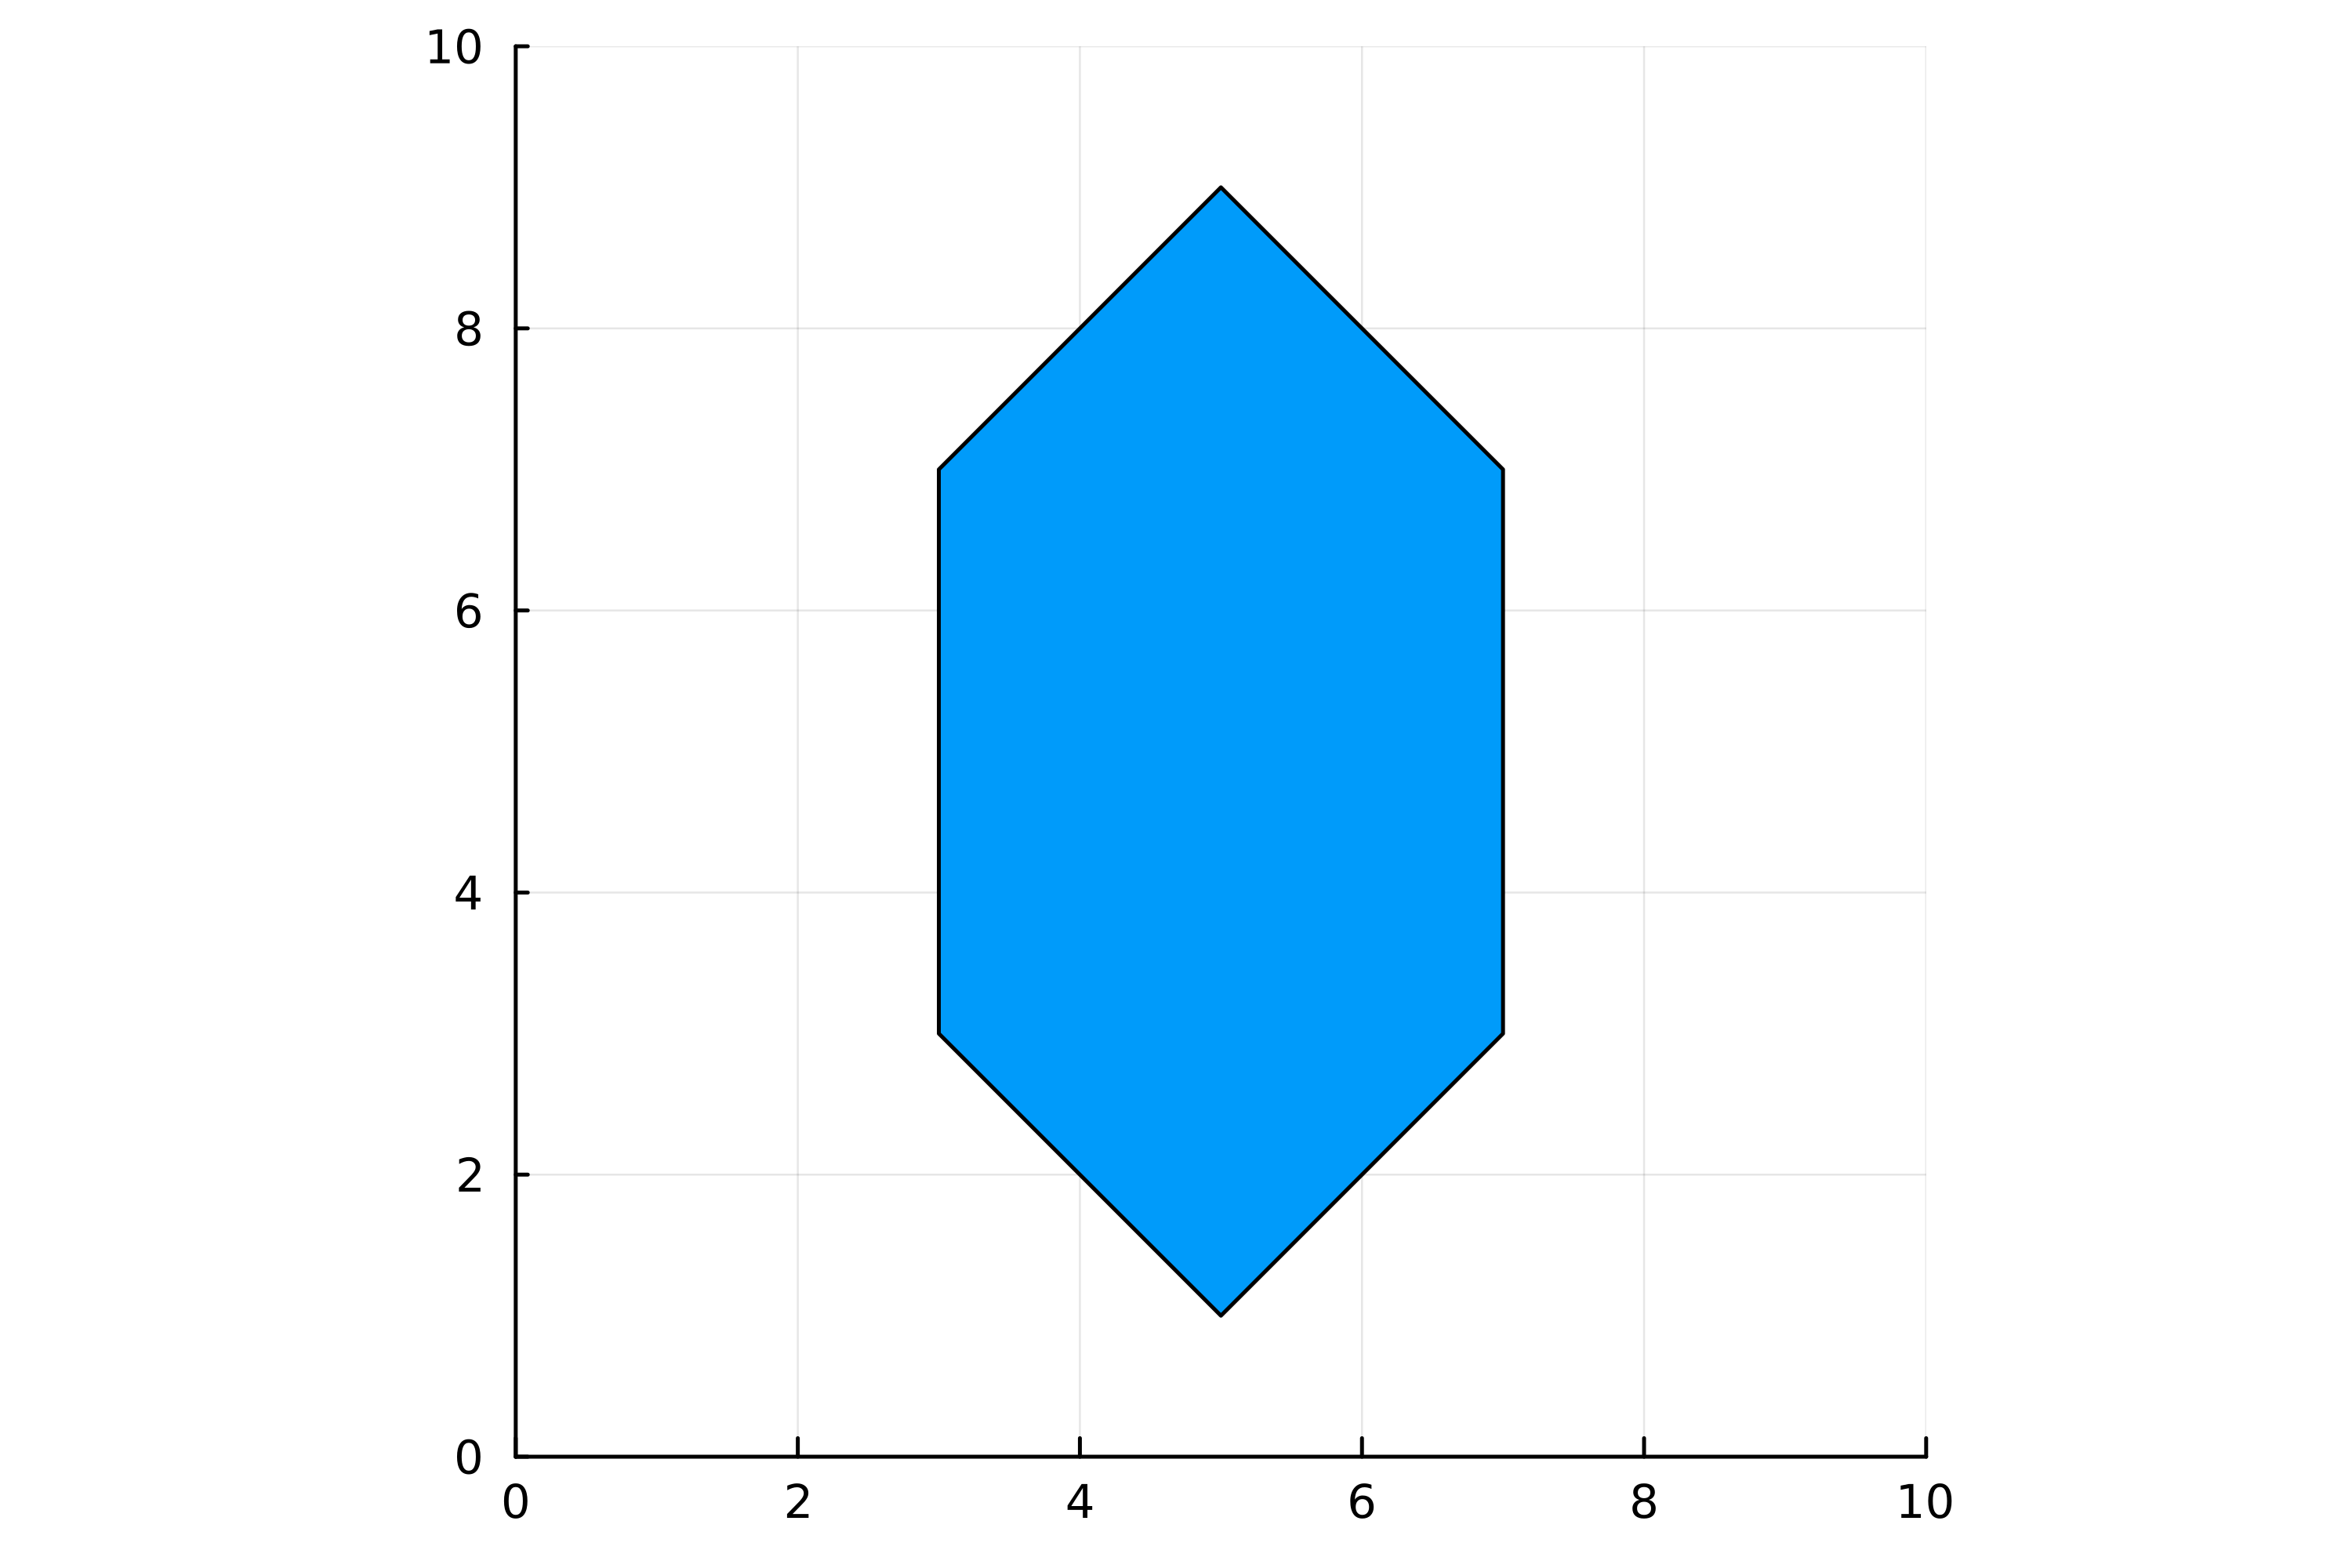
\includegraphics[width=\textwidth]{bachelors-thesis/model_illustrations/VertexModel.png}
		\caption{Another possibility to model cell forms are Vertex models. 
        An example of this is shown here. 
        This cell has six vertices. 
        In order to model cell deformations, one can define forces that act on each vertex separately and thus cause them to move in an according direction. }
	\end{subfigure}
	\caption{ To illustrate the models from the introduction, we can see a corresponding plot for each model. 
    In (a) and (b) the focus is more on the density distribution of the particles in $\Omega$. 
    The amount of particles is $N = 100$. The remaining sub figures (c) and (d) are concerned with the representation of cell shapes. 
    In all sub figures, the axes denote the spatial $x$ and $y$ coordinates. } 
	\label{fig:model_illus}
\end{figure}
In this thesis, we aim to derive forces that can be applied to our cell model and affect the diffusion behavior of the cell system, similar to the forces studied in \cite{Bruna2012} and \cite{Bruna2017}. \\

% transition to phase field models 
A limitation of the previous models is that they only considered spherical particles. 
In contrast, the next model we will introduce allows for particles of different shapes. 
In this thesis, we aim to develop models that can represent a wide range of shapes, as the shape of a cell can influence its diffusion behavior. 
Phase field models, for example, are capable of representing complex shapes, as demonstrated in the work of Happel and Voigt \cite{Happel2023}. \\
In this model, each cell is described by a two-dimensional phase field variable $\phi_i \in [-1, 1]$, which is a smooth function. 
The interior of the cell is represented by points $\vec{x} \in \Omega$ with positive values in $\phi_i$, while points with negative values are considered to be exterior. 
The cell wall is denoted by values of $\phi_i = 0$. \\
The dynamic for each $\phi_i$ is given by the equation
\begin{align}
	\dfrac{ \partial \phi_i}{ \partial t} + v_0(\textbf{v}_i \cdot \nabla_{\vec{x}} \phi_i) = \Delta_{\vec{x}} \dfrac{\delta F}{\delta \phi_i}, \qquad 1 \leq i \leq N \label{eq:phasefield},
\end{align}
where $\textbf{v}_i$ is a vector field used to incorporate activity, with a self propulsion strength $v_0$, $F$ is a free energy, and $\dfrac{\delta F}{\delta \phi_i}$ denotes the first variation.\\
The free energy $F$ arises from a sum of different energies, including shape preservation, cell interaction, and preservation of the codomain of $\phi_i$ to be $[-1, 1]$.
%%% TODO: MORE FOR PHASE FIELD MODEL 

% vertex based model 
A simpler approach for modeling diverse shapes in cell models is to use a vertex-based model, as used in \cite{Fletcher14}. 
Vertex models are a valuable tool in computational biology and biophysics for studying the biomechanics and behavior of cells and tissues. \\
In a vertex model of a cell, the cell's outline or boundary is approximated as a polygon, with the vertices of this polygon representing discrete points along the cell's boundary. 
Movements or transformations of the cell are given by forces that are applied on each vertex individually. \\
The cell dynamic in a vertex model is given by the equation
\begin{align}
	\eta \dfrac{d \vec{x}_i}{dt} = F_i, \qquad 1 \leq i \leq N \label{eq:vertexmodel}, 
\end{align}
where $\eta$ is a scaling factor and $F_i$ is the total force acting on $\vec{x}_i$. \\
Like in the phase field model, $F_i$ is a sum of different forces that define the cell behavior, such as the cell flexibility or the interaction with other cells. \\
Our new cell model shall be able to represent a wide range of shapes, similar to the phase field model in \cite{Happel2023} and the vertex model in \cite{Fletcher14}.

%%% TODO: work in missing papers 
%%% TODO: explain what was done in bachelor thesis 
%%% TODO: tell what happens in the following chapters 

